% ============================================================
% sections/methods.tex  モデルと実験方法（初稿 2026-10-25、用語を直した版 2026-10-25 23:55）
% 数字はプロジェクトの md にあるものだけ。【要確認】【結果待ち】は未確定。
% 版の番号と論文中の名前の対応は claude/論文_名前の対応表.md を参照。
% 用語（執筆メモ §3 の用語集と同じ）：重ね合わせ機構，視覚エンコーダ1・2，共有モジュール，
%   視覚予測器，特徴予測器，他者用モジュール，基準エンコーダ，自他一致度．「元論文」は使わない．
% ============================================================
\section{モデルと実験方法}\label{sec:method}

本研究では，Noguchi ら\cite{noguchi2022superposition}の重ね合わせ機構（superposition mechanism）を持つネットワークを，自分の価値に従って動いた経験の量だけが異なるデータで学習させ（段階I），その後に他者用のモジュールを学習させる（段階II）．
段階Iのモデルに対して実験1（自己側の見込み）と実験2（他者側への当てはめ）を，段階IIで実験3（他者用モジュールの学習）を，学習を伴わない評価として実験4（仮説の照合）を行う．
用いた条件を表\ref{tab:conditions}に，指標と事前登録の区別を表\ref{tab:metrics}に示す．

% ------------------------------------------------------------
\subsection{環境}\label{sec:env}

\begin{figure}[t]
  \centering
  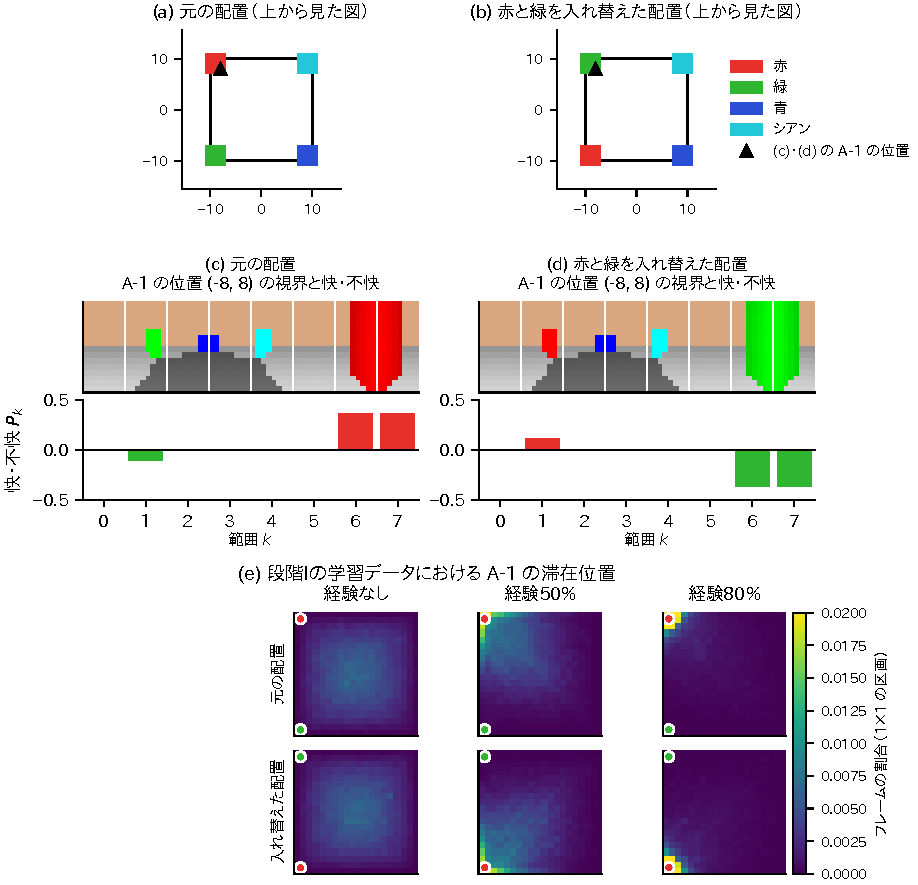
\includegraphics[width=\linewidth]{figs/env_conditions}
  % 図2：環境と条件。
  % (a) アリーナ（20×20）と四隅の外に置いた4色の立方体。元の配置と、赤と緑を入れ替えた配置を並べる。
  % (b) A-1 の全方位の視界（16×64）と、8つの範囲の快・不快 P_k（赤が見える範囲で正、緑で負）。
  %     元：data/result/v11/gate61/gate61_pleasure_views.png
  % (c) 段階Iの学習データでの A-1 の滞在位置。経験なし・経験50%・経験80% を横に並べる（元の配置と入れ替えの配置）。
  %     元：data/result/v13/gate61/gate61_v13_occupancy.png
  \caption{環境と条件．(a) アリーナとランドマークの配置．(b) 全方位の視界と方向ごとの快・不快．(c) 段階Iの学習データにおける A-1 の滞在位置．}
  \label{fig:env}
\end{figure}

環境は文献\cite{noguchi2022superposition}と同じ 20×20 の正方形のアリーナで，四隅の外側に赤・緑・青・シアンの立方体をランドマークとして置いた（図\ref{fig:env}(a)）．
エージェントは2体あり，学習するのは A-1 だけである．
A-2 は A-1 の視界に黒い立方体として映るだけで，A-2 自身の視界はネットワークに入らない．
A-1 は全方位カメラで $16\times64$ 画素の RGB 画像 $v_t$ を得る．
カメラは回転せず，画像の列は世界の方角に固定されている．
各ランドマークはどの位置から見てもちょうど16列（1象限）を占める．

文献\cite{noguchi2022superposition}との違いとして，エピソードごとに確率 1/2 で赤と緑のランドマークの位置を入れ替えた（以下，配置）．
配置はエピソードの中では変わらない．
入れ替えのない環境では，「赤の方へ動く」ことと「特定の場所へ動く」ことが学習データの上で区別できないためである．

各エピソードは 101 フレームからなる．
A-1 は1ステップに1の距離を動くか，休止（動く一歩ごとに確率 0.005 で始まり，10〜30 ステップ続く）の間は止まる．
ランダムに歩くときは文献\cite{noguchi2022superposition}と同じく，ランダムに選んだ目的地へ向かう．

\paragraph{方向ごとの快・不快}
A-1 の価値は，視界から毎ステップ計算する8次元の快・不快 $P_t=(P_{t,0},\dots,P_{t,7})$ として与えた（図\ref{fig:env}(b)）．
範囲 $k$ はカメラの境目に合わせた8列（列 $8k$〜$8k{+}7$）で，
\begin{equation}
  P_{t,k} = \frac{n^{\mathrm{like}}_{t,k} - n^{\mathrm{dislike}}_{t,k}}{128}
\end{equation}
とした．ここで $n^{\mathrm{like}}_{t,k}$，$n^{\mathrm{dislike}}_{t,k}$ は，マスクする前の $v_t$ で範囲 $k$ に見える好きな色と嫌いな色の画素数である．
A-1 にとって好きな色は赤，嫌いな色は緑である．
赤と緑はそれぞれ2つの範囲を占めるので，値が0以外になるのは範囲 0・1・6・7 だけで，範囲 2〜5（青とシアンの象限）は常に0である．
この値は人が計算して渡す生まれつきの信号であり，ネットワークが学ぶのは，この信号と自分の行動・視界の変化との関係である．

\paragraph{価値に従う一歩と経験の量}
価値に従う一歩は，学習を伴わない規則で作った．
視界の中の赤の画素の，列ごとの数を重みにした円周上の重心の方角へ，速さ1で進む．
アリーナの外に出る成分は消して壁に沿って進み，進めない場合（角にいる，赤が見えない）はランダムな一歩にした．
嫌いな色は行動には表れず，入力 $P_t$ の負の成分としてだけ表れる．

A-1 は休止していない各ステップで，確率 $p$ で規則の一歩を，残りでランダムな一歩をとる．
$p=0$ を経験なし条件，$p=0.5$ を経験50\%条件，$p=0.8$ を経験80\%条件と呼ぶ（表\ref{tab:conditions}）．
乱数はエピソードごとに設定し直し，同じエピソード番号では，配置・A-1 と A-2 の初期位置・休止の時刻が3条件で一致するようにした．
したがって条件の間で違うのは，休止していない一歩の向きと，その結果の位置と視界だけである．

学習データで赤から距離5以内にいるフレームの割合は，経験なし条件で約0.03，経験50\%条件で約0.33，経験80\%条件で約0.85であった．
経験80\%条件の A-1 は中央値14ステップで赤の角に着き，その後はほぼ角にとどまる．
角では規則の一歩が使えないため，実際に規則で動いた一歩は経験80\%条件で57\%（経験50\%条件で48\%）であった．
変えたのは規則の割合だけだが，学習データの位置の分布も大きく変わる点に注意が要る（\ref{sec:limitations}節）．

\paragraph{データ}
段階Iでは，A-2 は各エピソードの初めにランダムな位置に置かれ，動かない．
各条件で学習用 3000 エピソード，評価用 300 エピソードを集めた．
段階IIでは，A-1 はランダムに歩き，A-2 は A-2 自身の視界で同じ規則を用いて，一歩ごとに確率 0.5 で好きな色へ向かう．
A-2 が常に緑を好むデータ（緑好みデータ）と，エピソードごとに緑好き・赤好きが 1/2 で変わるデータ（好み混合データ）を，それぞれ学習用 3000・評価用 300 エピソード作った．

% ------------------------------------------------------------
\subsection{ネットワーク}\label{sec:network}

\begin{figure}[t]
  \centering
  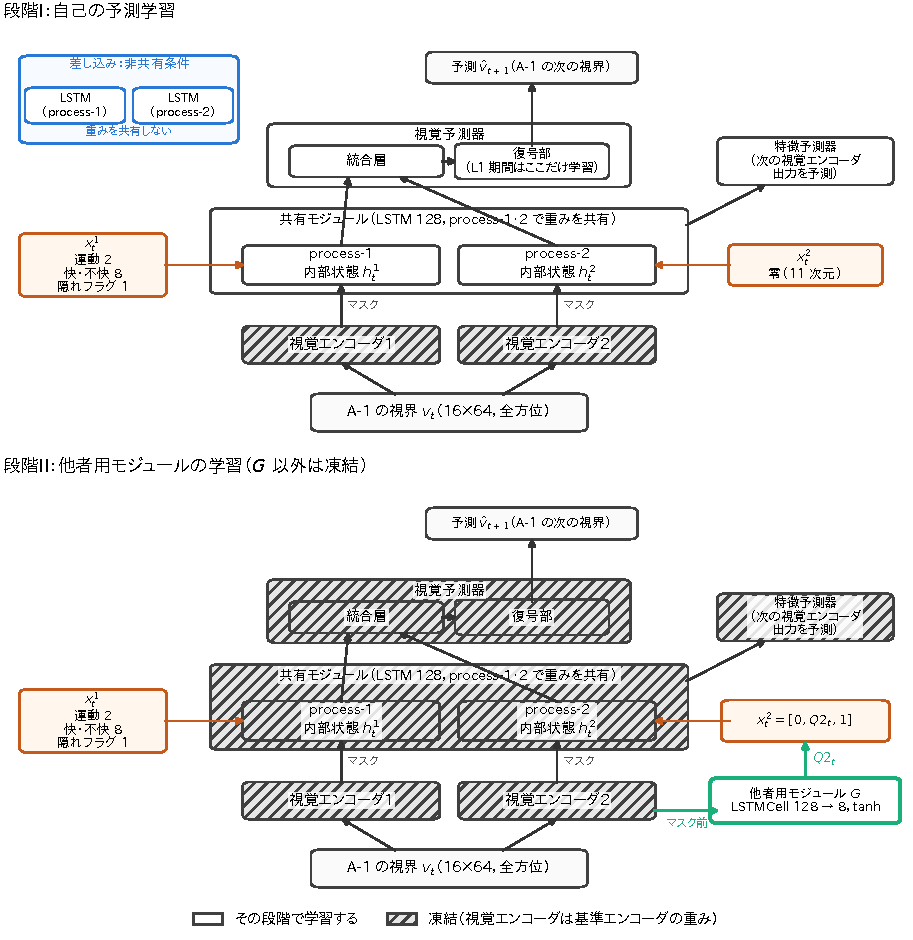
\includegraphics[width=\linewidth]{figs/network}
  % 図1：ネットワークと2段階の学習。
  % 左：段階I。A-1 の視界 v_t を視覚エンコーダ1・2（基準エンコーダで凍結、斜線）が読み、
  %     共有モジュール（LSTM 128）の process-1・process-2 に入る。process-1 には [運動 2, 快・不快 8, 隠れフラグ 1]、
  %     process-2 には零。視覚予測器が h^1, h^2 から v_{t+1} を予測する。特徴予測器も描く。
  % 右：段階II。他者用モジュール G（マスク前の視覚エンコーダ2の出力 → LSTMCell → 8次元）が Q2 を作り、
  %     process-2 の快・不快の枠に入れる（[0, Q2, 1]）。G 以外は凍結。
  % 差し込み：非共有条件では、共有モジュールの LSTM を process-1 用と process-2 用に分ける場所を示す。
  % 元：docs/figs/network_v11_v12.svg（v11 の部分を除き、非共有の差し込みを足す）
  \caption{ネットワークと学習の2段階．斜線は凍結したモジュールを表す．差し込みは非共有条件で分ける部分を示す．}
  \label{fig:network}
\end{figure}

\paragraph{重ね合わせ機構}
ネットワークは文献\cite{noguchi2022superposition}の重ね合わせ機構に従う（図\ref{fig:network}）．
同じ作りで重みの異なる2つの視覚エンコーダ（Visual Encoder-1，-2．3層の畳み込みと全結合層，層正規化）が，ともに A-1 の視界 $v_t$ を読み，特徴 $f^1_{v,t}$，$f^2_{v,t}$ を出す．
共有モジュール（Shared Module）は 128 ユニットの LSTM で，process-1 と process-2 は重みを共有し，内部状態 $h^1_t$，$h^2_t$ を別々に持つ：
\begin{align}
  (h^1_t, c^1_t) &= \phi_{\mathrm{shared}}\bigl(f^1_{v,t},\, x^1_t,\, h^1_{t-1}, c^1_{t-1}\bigr), \\
  (h^2_t, c^2_t) &= \phi_{\mathrm{shared}}\bigl(f^2_{v,t},\, x^2_t,\, h^2_{t-1}, c^2_{t-1}\bigr), \\
  \hat v_{t+1} &= \phi_{\mathrm{pred}}\bigl(h^1_t, h^2_t\bigr).
\end{align}
$\phi_{\mathrm{pred}}$ は2つの内部状態をまとめて次の視界を出す視覚予測器（Visual Predictor）である．
予測の対象は A-1 自身の次の視界 $v_{t+1}$ だけである．
文献\cite{noguchi2022superposition}と同じく，$h^1_t$，$h^2_t$ から次の視覚エンコーダの出力を予測する特徴予測器を置いた．
段階Iの学習中は，視覚エンコーダの出力を各ステップ確率 0.99 で零にする（視覚のマスク）．
視覚がない間も，入力を積み上げて状態を更新することを学ばせるためである．

\paragraph{process-1 の入力}
文献\cite{noguchi2022superposition}では $x^1_t$ は A-1 の運動 $m_t$（2次元）だった．
本研究では
\begin{equation}
  x^1_t = \bigl[\, m_t,\; P_t,\; b_t \,\bigr] \quad (11\ \text{次元})
\end{equation}
とした．$b_t$ は運動が隠れているかを示すフラグである．
運動は，5〜15 ステップの長さの「見える区間」と「隠れた区間」を交互に置いて隠す（$t\ge1$ の約48\%）．
隠れた区間では $m_t=0$，$b_t=1$ とし，$P_t$ を区間の最初の一歩の値に保つ．

運動を隠すのは，隠れた区間では次の視界を当てるために自分の動きを推し量る必要が生まれ，価値に従って動いた経験があれば「快の高い方へ動いている」と推し量る理由が生まれるからである．
$P_t$ を保つのは，その変わり方から自分の動きを読み取れてしまうことを防ぐためである．
フラグ $b_t$ を入れるのは，休止でも $m_t=0$ になるため，「動いていない」と「動きが分からない」を区別できるようにするためである．
段階Iでは process-2 の入力 $x^2_t$ は11次元すべて零とした（文献\cite{noguchi2022superposition}と同じく A-2 は動かない）．

\paragraph{基準エンコーダ}
2つの視覚エンコーダは，すべての条件で，文献\cite{noguchi2022superposition}の学習設定（運動を入力，入れ替えなしの環境，1000 エピソード）で我々が一から再現学習した重み（以下，基準エンコーダ）に固定した．
基準エンコーダを用いた再現モデルでは，$h^1$ から A-1 の位置が $R^2=0.977$，$h^2$ から A-2 の位置が 0.973 で読め，文献\cite{noguchi2022superposition}の図5に当たる他者視点の取り出し（視覚エンコーダ2の出力を，視覚エンコーダ1の出力から視界を復元するよう学習した復号器に通すと，A-2 から見た視界が得られる）がマージン +0.091 で成り立つ．
また，視覚エンコーダ2が A-1 の視界から作る符号と，視覚エンコーダ1に A-2 の視界を入れたときの符号のコサイン類似度（以下，自他一致度）は 0.80 である．

基準エンコーダに固定したのは，運動以外の入力（快・不快と運動の遮蔽）を加えて視覚エンコーダごと一から学習すると，自他一致度が 0.18〜0.27 にとどまったためである（付録\ref{app:encoder}）．
基準エンコーダはすべての条件で同じで，快・不快や好みを一度も見ていない．
そのため経験の効果は，共有モジュール・視覚予測器・特徴予測器にだけ生まれる．
一方で，自他を同じ符号で表す性質は学んだものではなく与えたものであり，本研究が問えるのは「その土台がある上で，価値の経験が何を生むか」までである（\ref{sec:limitations}節）．

\paragraph{非共有条件}
共有の役割を確かめるため，共有モジュールの LSTM を process-1 用と process-2 用の2つに分けたモデルを作った（非共有条件，経験80\%のデータで学習）．
層正規化と特徴予測器は分けていない．
process-2 用の LSTM は process-1 用の写しから始めるので，初期値・バッチの順・運動を隠す区間は同じ組の経験80\%条件と一致し，両者を同じエピソードで対にして比べられる．
段階Iでは process-2 の入力が常に零なので，非共有条件では process-2 の快・不快を受ける入力の重みが一度も学習されない．
したがって，非共有条件で他者側の効果が出ないことは構成からほぼ予想でき，この比較は「他者側へ届く経路が共有以外にないこと」の確認として位置づける．

% ------------------------------------------------------------
\subsection{学習}\label{sec:training}

\paragraph{段階I（自己の予測学習）}
文献\cite{noguchi2022superposition}の手順に従い，前半の 200 エポック（MSE 期間）は次の視界の二乗誤差で共有モジュール・視覚予測器・特徴予測器を学習し，後半の 200 エポック（L1 期間）は絶対誤差で視覚予測器だけを学習した．
% 【要確認】L1 期間に学習する範囲：コードでは vision_decoder_module だけが変わる（v14 ログ §20）。
%   これが h^1・h^2 をまとめる全結合層を含む視覚予測器全体に当たるかを Claude Code で確かめる。
視覚エンコーダは全期間で凍結した．
最適化は AdamW（学習率 $10^{-3}$，重み減衰 0.01，バッチ 10）とした【要確認：段階I本番の設定ファイルの値】．
特徴予測器への入力と目標は勾配を止めてあり，段階Iでは特徴予測器だけがこの損失で学習される（文献\cite{noguchi2022superposition}と同じ）．

\paragraph{段階II（他者用モジュールの学習）}
文献\cite{noguchi2022superposition}の Motion Generator と同じ構成の他者用モジュール $G$ を加えた．
$G$ はマスクする前の視覚エンコーダ2の出力（64次元）を LSTMCell（128 ユニット）と全結合層で受け，tanh を通した8次元の出力 $Q2_t$ を作る．
これを $x^2_t = [\,0,\, Q2_t,\, 1\,]$ として process-2 の快・不快の枠に入れる．
つまり，他者の運動は「隠れている」とし，快・不快の枠だけを $G$ に埋めさせる．
運動の枠に $G$ の出力を入れないのは，入れると $G$ は他者の動きそのものを書き込むことを覚え，好みを表す理由がなくなるためである．

学習は文献\cite{noguchi2022superposition}の Motion Generator の学習手順に合わせた．
$G$ 以外はすべて凍結し，視覚は $t>0$ で process-1・process-2 とも隠す．
process-1 には運動を隠さずに入れる．
損失は A-1 の次の視界の絶対誤差と特徴予測の誤差で，後者の勾配は $h^2$ を通って $G$ に届く．
AdamW（学習率 $10^{-3}$，重み減衰 0.01，バッチ 10）で 200 エポック学習した．

他者用モジュールの構成は4通り試した（表\ref{tab:conditions}）．
(i) 自由出力モジュールは上のとおり8次元を自由に出す．
(ii) 形制限モジュールは，出力を自分が経験した快・不快の形に限る（範囲 2〜5 は0，範囲 0・1 と 6・7 は逆の符号で，どちら側が快いかを1つの符号で決め，範囲ごとの強さはモジュールが決める）．
(iii) 他者遮蔽学習は，(ii) のモジュールを，学習データの入力の視界から A-2 を 10〜30 ステップの区間で消して学習する（予測の正解は A-2 が写った視界のまま）．
(iv) 1ビットモジュールは，出力をスカラー $u_t\in(-1,1)$ だけにし，$Q2_t = u_t\, c^{+}$ とする．
$c^{+}$ は範囲 6・7 が快い固定の形で，段階Iの学習データの $|P|$ の範囲ごとの平均から作った $c^{+}=(-0.104,-0.127,0,0,0,0,+0.127,+0.104)$ である．
(ii) と (iii) は，(i) の結果を見た後に設計した探索として扱う（表\ref{tab:metrics}）．
各構成の詳しい結果は付録\ref{app:component}に示す．

\paragraph{組}
同じシードで学習した各条件のモデルを一つの「組」とする．
同じ組の中では，初期値・バッチの順・運動を隠す区間が条件の間で一致し，違うのは学習データだけである．
経験なし条件のモデルは，データの一致と，学習し直したときの重みのビット単位の一致を確かめたうえで，経験50\%条件と経験80\%条件の両方の相手として用いた．
事前登録した判定は本番の3組（組1〜3）で行い，予備として登録した組4と，後から追加した組5・6も，事前登録に従ってすべて報告し除外しない．
組5・6 では段階Iの学習と，それを用いる実験1，実験2（真値条件の評価を除く），実験4を行った．
非共有条件は組1〜3，段階IIは組1〜4（1ビットモジュールは組1〜3）で行い，実験4は全6組に当てた（主の判定は本番の3組）（表\ref{tab:conditions}）．

\begin{table}[t]
  \centering
  \caption{条件と組の一覧}
  \label{tab:conditions}
  % paper/tables/conditions.tex -- generated by analyze/paper/tables_paper.py; sources in paper/tables/README.md
\begin{tabular}{@{}p{0.14\linewidth}p{0.24\linewidth}p{0.19\linewidth}p{0.16\linewidth}p{0.13\linewidth}@{}}
\toprule
条件 & A-1 が規則で動く割合 $p$ & 共有モジュールの LSTM & 段階Iと実験1・2の組 & 実験4の組 \\
\midrule
経験なし条件 & 0 & 共有 & 組1〜6 & 組1〜6 \\
経験50\%条件 & 0.5 & 共有 & 組1〜6 & 組1〜6 \\
経験80\%条件 & 0.8 & 共有 & 組1〜6 & 組1〜6 \\
非共有条件 & 0.8 & process-1 用と process-2 用に分ける & 組1〜3 & 組1〜3 \\
\midrule
他者用モジュール（段階II） & 出力の形 & 学習データの入力の視界 & 段階Iの条件と組 & 扱い \\
\midrule
自由出力モジュール & 8次元を自由に（tanh） & そのまま & 経験なし・50\%・80\%，組1〜4 & 経験50\%：事前登録した主，経験80\%：探索 \\
形制限モジュール & 自分が経験した快・不快の形（範囲2〜5は0，範囲ごとの強さは自由） & そのまま & 経験なし・50\%，組1〜4 & 探索 \\
他者遮蔽学習 & 形制限モジュールと同じ & A-2 を10〜30ステップの区間で消す & 経験なし・50\%，組1〜3 & 探索（新しい仮説を事前登録） \\
1ビットモジュール & スカラー $u_t$（$Q2_t=u_t\,c^{+}$） & そのまま & 経験なし・50\%・80\%，組1〜3 & 事前登録 \\
\midrule
\multicolumn{5}{@{}p{0.97\linewidth}@{}}{注：付録実験Aの好み切替条件（A-1 の好きな色をエピソードごとに赤・緑から選ぶ，規則で動く割合 0.5，共有，組1〜3）は表に含めない．} \\
\bottomrule
\end{tabular}

  % 表1：条件の一覧（Claude Code が .tex で作る）。
  % 行：経験なし条件／経験50%条件／経験80%条件／非共有条件（＋付録の好み切替条件は脚注で触れる）。
  % 列：A-1 が規則で動く割合 p、共有 LSTM の有無、段階Iの組（組1〜6 か 組1〜3）、段階IIの組、実験4の組（組1〜6、非共有は組1〜3）。
  % 下段：段階IIの他者用モジュール4通り（自由出力／形制限／他者遮蔽学習／1ビット）。出力の形、学習データの視界、組の数、扱い（事前登録・探索）。
  % 出典：claude/論文_名前の対応表.md §2・§3・§5
\end{table}

% ------------------------------------------------------------
\subsection{評価}\label{sec:evaluation}

\paragraph{判定の共通の規則}
各モデルについて，学習の最後の5つのチェックポイント（最終5点）で評価した（段階Iの自分側の指標は MSE 期間，他者側の指標は L1 期間の最終5点）．
各点で，経験ありの値と組の差（経験あり $-$ 経験なし）の 95\% 信頼区間を，同じエピソードで対にしたブートストラップ（1000回）で求めた．
経験ありの値が仮説の向きで，かつ組の差の信頼区間が0を含まない点が5点中3点以上ならその組は合格とし，3組中2組以上（4組では3組以上）で合格とした．
評価は同じチェックポイントを2回流し，結果がビット単位で一致することを確かめた．
これらの判定の基準は計算の前に記録した（事前登録）．

組をまたいだ比較では，各組の最終5点の平均を1つの値とし，組どうしを対にした差の平均と $t$ 分布による 95\% 信頼区間（6組で自由度5）を求めた．
これは事前登録していない記述的な分析である．
各指標が事前登録したものか，結果を見た後に定義したものかを表\ref{tab:metrics}に示す．

\begin{table}[t]
  \centering
  \caption{指標の定義と事前登録の区別}
  \label{tab:metrics}
  % paper/tables/metrics.tex -- generated by analyze/paper/tables_paper.py; sources in paper/tables/README.md
\begin{tabular}{@{}p{0.17\linewidth}p{0.33\linewidth}p{0.15\linewidth}p{0.26\linewidth}@{}}
\toprule
指標 & 何を測るか & 評価データ／点 & 位置づけ \\
\midrule
\multicolumn{4}{@{}l}{\textbf{自分側の見込み}} \\
自己位置の追跡 & 運動が見えるステップで $h^1$ から A-1 の位置を線形回帰で読む決定係数（0.80 以上を前提とする） & 共通／MSE & 事前登録した前提 \\
価値と行動・色の結びつき（3指標） & 運動が隠れたステップで予測が赤の方へ一歩動いた視界に寄るか（定義は補足資料 S13） & 共通／MSE & 事前登録した主 \\
自己側の積み上がり $g$ & 運動と視覚を止めた15ステップで予測が赤の方へだけ進み続ける傾きの差 & 共通／MSE & 事前登録した主 \\
快・不快への依存 $d_P$ & 快・不快を保ったときの $g$ と，符号を反転して保ったときの $g$ の差の半分 & 共通／MSE & 事前登録（符号無作為条件との比較）．好み切替条件では事前登録外 \\
\midrule
\multicolumn{4}{@{}l}{\textbf{他者側への転用}} \\
他者側の符号応答 G5b & process-2 の1つの範囲に $\pm a$ を入れたときの予測の中の A-2 のずれの差 & 共通（A-2 静止）／L1 & 事前登録した主 \\
符号に従う分 & 本当の快・不快を保った傾きと符号を反転して保った傾きの差の半分 & 緑好み，好み混合／L1 & 定義は事後（組1〜4）．組5・6 の経験の比較と符号無作為条件との比較は事前登録 \\
他者側の積み上がり G5a & 本当の快・不快を保ったときの予測の中の A-2 の傾き（戻る動きが混ざる） & 緑好み，好み混合／L1 & 事前登録した関門．結果を見た後に副へ \\
真値条件の $\Delta$ & process-2 に本当の快・不快を入れたときと零を入れたときの他者側の特徴予測の誤差の差 & 緑好み，好み混合／L1 の最後 & 事前登録外（悪化は予想外）．規則の確率の比較と符号無作為の組1〜3 は事前登録 \\
\midrule
\multicolumn{4}{@{}l}{\textbf{他者用モジュールの見分け}} \\
入れ替え応答 T2 & $t=50$ で赤と緑を入れ替えたとき $Q2$ が新しく緑が見える範囲へ移るか & 緑好み／段階II & 事前登録した主 \\
好み差応答 T5 & 位置をそろえた緑好き・赤好きの A-2 で $Q2$ が好みに応じて違うか & 緑好み，赤好み／段階II & 事前登録した主 \\
好み追従率（1ビット） & 好みと方角が食い違うエピソードで $u_t$ が好みに従う割合 & 好み混合／段階II & 事前登録（経験80\%），結果を見た後の確認（経験50\%） \\
\midrule
\multicolumn{4}{@{}l}{\textbf{照合}} \\
正解率 BA & 2つの候補のうち予測誤差の和が小さい方を選んだ正解率（配置と好みの4つの組み合わせの平均） & 好み混合／自己視界：L1，他者特徴：MSE & 事前登録した主（自己視界基準），副（他者特徴基準） \\
好み追従率 & 好みと方角が食い違う88エピソードで選択が好みに従う割合 & 好み混合／他者特徴：MSE & 事前登録（経験50\%の結果の後，経験80\%の結果の前） \\
方角だけの基準 & A-2 の $t=1$〜50 の変位の方角で選んだときの BA（データだけで決まる） & 好み混合 & 事前登録外の記述 \\
\midrule
\multicolumn{4}{@{}l}{\textbf{全体}} \\
組をまたいだ統計 & 各組の最終5点の平均を1つの値とし，組を対にした差の平均と $t$ 分布の95\%信頼区間 & --- & 事前登録外の記述（符号無作為条件の6組は判定として登録） \\
\midrule
\multicolumn{4}{@{}p{0.97\linewidth}@{}}{評価データ：共通＝共通テスト（経験なし条件の評価用データ），緑好み・赤好み・好み混合＝それぞれの評価用データ．チェックポイント：MSE・L1＝段階Iの MSE 期間・L1 期間の最終5点，L1 の最後＝段階Iの L1 期間の最後のチェックポイント（エポック 200），段階II＝段階IIの最終5点．} \\
\bottomrule
\end{tabular}

  % 表2：指標の一覧（Claude Code が .tex で作る）。
  % 列：実験、指標の名前、何を測るか（一行）、評価データ、チェックポイント、位置づけ。
  % 位置づけの区分：事前登録した主／事前登録した副／事後に定義（どの組で事前登録したかも書く）／事前登録外の記述／探索。
  % 行：G1（前提）、G2（M1(c)・M1(d)・色の基準。定義は付録E）、G3、G5b、符号に従う分（組1〜4 は事後、組5・6 は事前登録）、
  %     G5a（事前登録の関門だったが副に下げた）、T3（真値条件）、T2、T5、BA、好み追従率、方角だけの基準、組をまたいだ t の信頼区間。
  % 出典：claude/論文_名前の対応表.md §8、v13_summary.md §3.1・§11
\end{table}

\paragraph{実験1：自己側の見込み}
前提として，運動が見えるステップで $h^1$ から A-1 の位置を線形回帰で読む決定係数（自己位置の追跡）が 0.80 以上であることを確かめた．
また，運動が隠れたステップで，予測が「赤の方へ一歩動いた場合の視界」に寄るか（価値と行動・色の結びつき）を確かめた（定義は付録\ref{app:gates}）．

主の指標は，入力を止めたときの自己側の積み上がり $g$ である．
共通テスト（経験なし条件の評価用データ）の各エピソードで，$t=20$ から15ステップ，運動と視覚を隠し（$b_t=1$），快・不快を $t=20$ の値に保つ．
各ステップ $k$ の予測を，$t=20$ の位置から色 $X$ のランドマークの方へ $d=0,\dots,10$ 歩動いた場合の視界（シミュレータで描き直したもの）と比べ，最もよく合う $d$ を $d^{*}_{X}(k)$ とする．
$d^{*}_{X}(k)$ を $k$ に対して直線で合わせた傾きを $s_X$ とし，
\begin{equation}
  g = s_{\text{赤}} - \tfrac{1}{3}\bigl(s_{\text{緑}} + s_{\text{青}} + s_{\text{シアン}}\bigr)
\end{equation}
とした．
運動が分からないときに予測が赤の方へだけ進み続ければ $g>0$ になる．
これは内部状態から位置を読み出すのではなく，モデル自身の予測で測る量である．

\paragraph{実験2：他者側への当てはめ}
段階Iのモデルの process-2 に快・不快を入れ，予測画像の中の A-2 がその向きに動くかを調べた．
予測画像からの A-2 の位置は，背景より暗い画素の列ごとの量から方角と距離を求めて読み取った（距離の換算は本当の視界で合わせた）．

主の指標（事前登録）は他者側の符号応答 G5b である．
A-2 が静止した共通テストで，$t=0$〜19 は通常どおり流し，$t=20$〜29 の10ステップ，process-2 に $[\,0,\,P^{(k,\pm)},\,1\,]$ を入れる．
$P^{(k,\pm)}$ は範囲 $k$ だけに $\pm a$（$a=0.28$）を入れ，ほかを0にしたものである．
10ステップ後の予測の中の A-2 の位置の，快・不快を0にした場合からのずれを $\Delta_k(\pm a)$ とし，
\begin{equation}
  \mathrm{G5b} = \frac{1}{8}\sum_{k=0}^{7} \bigl(\Delta_k(+a) - \Delta_k(-a)\bigr)\cdot u_k
\end{equation}
とした．$u_k$ は範囲 $k$ の方角の単位ベクトルである．
同じ入力の履歴から $+a$ と $-a$ の差をとるので，A-2 をもともとどこに置いていたかに左右されない．
ただし，静止した A-2 に1つの範囲だけの人工的な入力を入れる検査であり，A-2 の本当の好みは使っていない．

二つ目の指標は，A-2 の本当の快・不快を用いる「符号に従う分」である．
段階IIの評価用データで，$t<20$ は process-2 に A-2 の視界から計算した本当の快・不快 $P^{A2}_t$ を入れ，$t=20$ から15ステップは $P^{A2}_{20}$ に保つ．
予測の中の A-2 の位置を，A-2 の好きな色の方向とほかの3色の方向に射影した傾きの差を $g_{\mathrm{other}}$ とする．
同じ手順で保つ値の符号を反転した場合（$-P^{A2}_{20}$）の $g_{\mathrm{other}}$ と比べ，
\begin{equation}
  \text{符号に従う分} = \tfrac{1}{2}\bigl(g_{\mathrm{other}}(P^{A2}_{20}) - g_{\mathrm{other}}(-P^{A2}_{20})\bigr)
\end{equation}
とした．
入れた快・不快の向きに従う動きは符号の反転で向きが変わり，それ以外の動き（止める前に置いた位置から本当の位置へ戻る動きなど）は変わらないので，差によって前者だけが残る．
緑好みデータと好み混合データの両方で測った．

この指標は，事前登録した関門 G5a（保った快・不快のもとでの傾き $g_{\mathrm{other}}$ そのもの）に，戻る動きが混ざることが分かった後に定義した．
組1〜4 では結果を見た後に定義した指標であり，事前登録してから計算したのは組5・6 だけである．
G5a は副として付録に示す．

最後に，他者の本当の快・不快を与えたときの予測を調べた．
段階IIの評価用データで，process-2 に $[\,0,\,P^{A2}_t,\,1\,]$ を入れる条件（真値条件）を作り，他者側の特徴予測の誤差を，零を入れた場合と比べた（T3）．
この値は段階Iのモデルだけで決まり，他者用モジュールの学習によらない．
なお，段階Iの process-2 には零しか入らないので，真値条件の入力は段階Iのモデルにとって学習で見ていない入力である．

\paragraph{実験3：他者用モジュールの学習}
他者用モジュールが他者の好みを書き出すかを，事前登録した2つの見分けで調べた．
入れ替え応答 T2 は，緑好きの A-2 のエピソードで，$t=50$ に赤と緑だけを入れ替えたときに（$t\le49$ は入れ替えない場合と完全に同じで，$t=50$ でも A-1 と A-2 の位置は同じ），$Q2$ の値が新しく緑が見える範囲へ移るかを測る：
\begin{equation}
  s_{T2} = \bigl[Q2^{\mathrm{swap}}_{50}(\mathcal{G}') - Q2^{\mathrm{swap}}_{50}(\mathcal{G})\bigr]
         - \bigl[Q2^{\mathrm{noswap}}_{50}(\mathcal{G}') - Q2^{\mathrm{noswap}}_{50}(\mathcal{G})\bigr].
\end{equation}
$\mathcal{G}$ は入れ替え前に緑が見える2範囲，$\mathcal{G}'$ は入れ替え後に緑が見える2範囲で，$Q2(\cdot)$ はその範囲の平均である．
好みを表していれば $s_{T2}>0$，位置だけを伝えていれば $s_{T2}\approx0$ になる．
好み差応答 T5 は，同じ配置の中で，A-2 の位置が1.0以内かつ A-1 の位置が3.0以内の緑好きと赤好きのフレーム（$t\ge20$）を近いものから1対1で組にし，$[Q2(\text{緑の範囲}) - Q2(\text{赤の範囲})]$ の差（緑好き $-$ 赤好き）を平均したものである．
好みを表していれば正になる．
大きさの目安として，$Q2$ の代わりに A-2 の本当の快・不快を入れた値（T2 で +0.60，T5 で +0.42）を並べる．

他者用モジュールが何を書いているかの手がかりとして，$Q2$ と $P^{A2}$ の相関，$Q2$ の分散のうち範囲 2〜5（本当の快・不快が常に0の範囲）が占める割合，T3 で生成した $Q2$ と真値条件の誤差を比べた．
1ビットモジュールでは，好みと方角が食い違うエピソードで $u_t$ が好みに従う割合（下記）も測った．

\paragraph{実験4：仮説の照合}
学習を伴わない手続きで，段階Iのモデルに他者の好みの候補を入れて予測を比べた．
好み混合データの評価用 300 エピソードで，process-2 に $[\,0,\,c,\,1\,]$ を全ステップ入れ，$c\in\{c^{+},c^{-}\}$（$c^{-}=-c^{+}$，範囲 0・1 が快い形）の2通りで流す．
目標のフレーム1〜$T$（主は $T=50$）の予測誤差の和が小さい方を選び，A-2 の好きな色が範囲 6・7 にあるエピソードでは $c^{+}$，範囲 0・1 にあるエピソードでは $c^{-}$ を正解とする．
候補は A-2 の位置を使わない定数なので，他者用モジュールを介して位置を伝える経路はない．
主の誤差は A-1 の視界の予測誤差（自己視界基準，L1 期間の最終5点），副は他者側の特徴予測の誤差（他者特徴基準）とした．
他者特徴基準の値は視覚予測器だけを学習する L1 期間には変わらないので，MSE 期間の最終5点で数えた．
主の指標は，配置と好みの4つの組み合わせごとの正解率の平均（balanced accuracy，BA）である．
共有の役割を確かめるため，経験80\%条件と非共有条件を同じエピソードで対にして比べた（組1〜3）．
主の判定は本番の3組で行い，組4〜6 は事前登録に従って除外せず，全6組で何組が成り立つかを頑健さとして示す．

A-2 の好みは，A-2 がその間に進んだ方角とも結びついているので，正解率だけでは「好み」と「方角」を区別できない．
そこで，A-2 の $t=1$〜50 の変位が範囲 6・7 の方向に寄っていれば $c^{+}$，そうでなければ $c^{-}$ とする「方角の正解」を作った．
これは好みの正解と全体の 0.707 で一致する（データだけで決まる値）．
両者が食い違う 88 エピソードで，選択が好みの側に従う割合（好み追従率）を求め，その 95\% 信頼区間の下限が 0.5 を上回る点が最終5点のうち3点以上ある組を「好みを区別している」，そうでない組を「方角を区別している」と書くことを，経験80\%条件の結果を見る前に事前登録した．
この条件は経験50\%条件の結果を見た後に作ったものである（表\ref{tab:metrics}）．
比較の基準として，方角の正解をそのまま選択とする「方角だけの基準」の BA を並べる【要確認：方角だけの基準の BA は md にない。Claude Code で出す】．
方角だけの基準は A-2 の本当の位置を使うのに対し，モデルが使うのは A-1 の視界だけである．
